\chapter{Graph Simplification}
Once we started generating graphs, we noticed that the graphs we generated were nearly unusable for all but the simplest programs. These graphs were rendered as giant nests of events, with each event having many edges in different parts of the codebase. To improve the clarity of the graphs, we implemented a FSM miner, a module system, and node-grouping techniques to simplify them.

\section{Synoptic}
The first tool we used to simplify the graph was Synoptic, a finite state machine (FSM) miner. Developed by the University of Washington, Synoptic is described in their paper "Leveraging Existing Instrumentation to Automatically Infer Invariant-Constrained Models" \cite{synoptic}. Synoptic accepts a series of events that it uses to refine the graph. First, it creates a compact model where each node exists only once and is connected to all of the nodes that directly followed or preceeded it. Then Synoptic and then mines invariants from the graph. In this context, an invariant is a statement such as "x is always followed by y", "x always precedes y", or "x is never followed by y". By mining invariants, Synoptic is able to refine the graph and seperate nodes that are otherwise abiguous into multiple copies of the same node that represent different execution paths. This results in graphs with many more nodes but with each node follows a clear and unique execution path. Consider the graph in figure \ref{fig:graph} where you can see how synoptic was able to break apart \texttt{print} and \texttt{init} in \texttt{count\_to} into two seperate sets of nodes depending on whether or not they were called from \texttt{count to 10} or \texttt{count to 7}

\section{Modules}
\label{sec:modules}
Secondly, we employed a module system for events in order to achieve greater organization and simplicity. This system allows for the creation of namespaces, similar to popular programming languages. For example, instead of naming two "entry" points of functions as func1\_entry and func2\_entry, we can define a module with a unique name and a single parent, such as "add" being a child of "util". In this case, the entry point of "add" can be specified as "add::entry" and the entry point of another function like "print" can be specified as "print::entry".

This might look like the following in code:

\begin{verbatim}

#include <stdio.h>
// [[{type:"module", name:"util"}]]
// [[{type:"module", name:"print", parent_module:"util"}]]
// [[{type:"module", name:"add", parent_module:"util"}]]

int increment(int a){
    // Define a start event that gets expanded into ::util::add::entry
    // [[{type:"event", name:"add::entry"}]]
    a = a+1;
    return a;
}
void print_num(int a){
    // Define a start event that gets expanded into ::util::print::entry
    // [[{type:"event", name:"print::entry"}]]
    printf("val: %d\n", a);
}

int main(){
    // [[{type:"event", name:"::entry"}]]
    int a = increment(2);
    print_num(a);
    // [[{type:"event", name:"::exiting after printing the num"}]]
    return 0;
}
\end{verbatim}
\begin{figure}[!ht]
    \centering
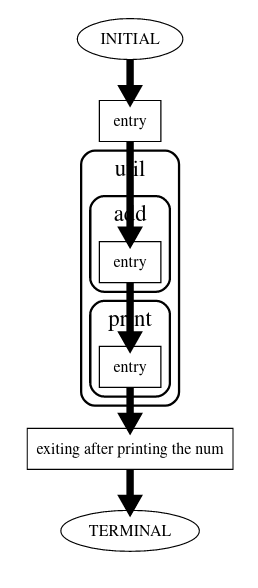
\includegraphics[scale=0.5]{modules}
    \caption{Graph of simple module system}
    \label{fig:modules}
\end{figure}

As you can see in figure \ref{fig:modules}, this sample code generated a simple graph containing multiple entry nodes all grouped into multiple different modules. This example is very contrived however it demonstrates multiple aspects of the module system. We can also see in figure \ref{fig:modules-collapsed} how these modules can be collapsed to simplify and hide complexity in the graph


\begin{figure}[!ht]
\centering
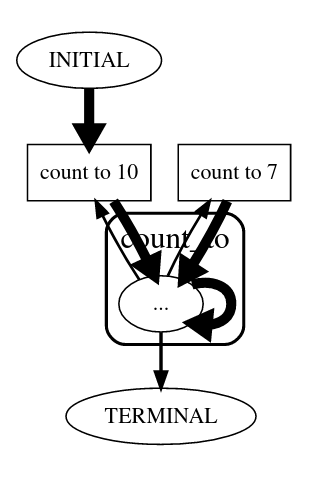
\includegraphics[scale=0.5]{modules-collapsed}
\caption{A collapsed module for a different program}
    \label{fig:modules-collapsed}
\end{figure}

We recommend keeping the number of modules to a minimum in order to prevent complicated and difficult-to-understand graphs. With many modules, graphviz is more constrained during graph layout and this can cause the creation of many extra extremely long edges. However, careful placement of a few modules can make the graph much more legible and easily navigable. 


\section{Grouping Strictly Sequential Nodes}
Finally, we used the idea of grouping nodes that are strictly sequential to simplify the graphs in our project. We define strictly sequential nodes A and B as having the only edge out of A directed to B and the only edge into B coming from A. Similarly, a set of nodes (A,B,C) is strictly sequential if A and B are strictly sequential and B and C are also strictly sequential. This technique is particularly useful for Synoptic graph simplification because Synoptic produces a large number of nodes and this helps to constrain and visually separate the graph. These groups are automatically highlighted to the user with a dotted border. We created figure \ref{fig:seq-on-off} to show the effect of sequential grouping. These are two photos of the same graph, one with grouping enabled, and the other with it disabled. In this case, the grouping allows the user to quickly see the relationships between nodes that were otherwise hidden due to how they were displayed in the image on the left.


\begin{figure}[!ht]
\centering
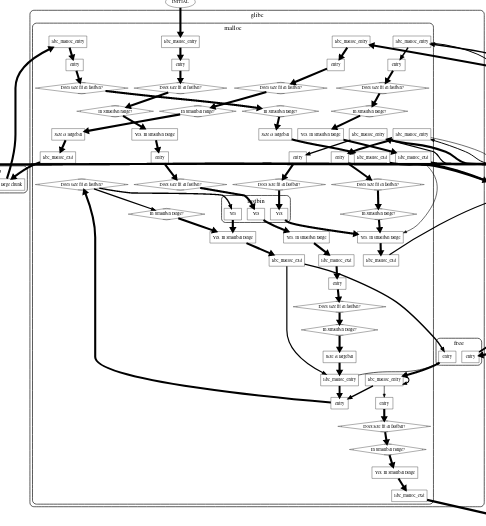
\includegraphics[scale=0.3]{simplification-sequential-off}
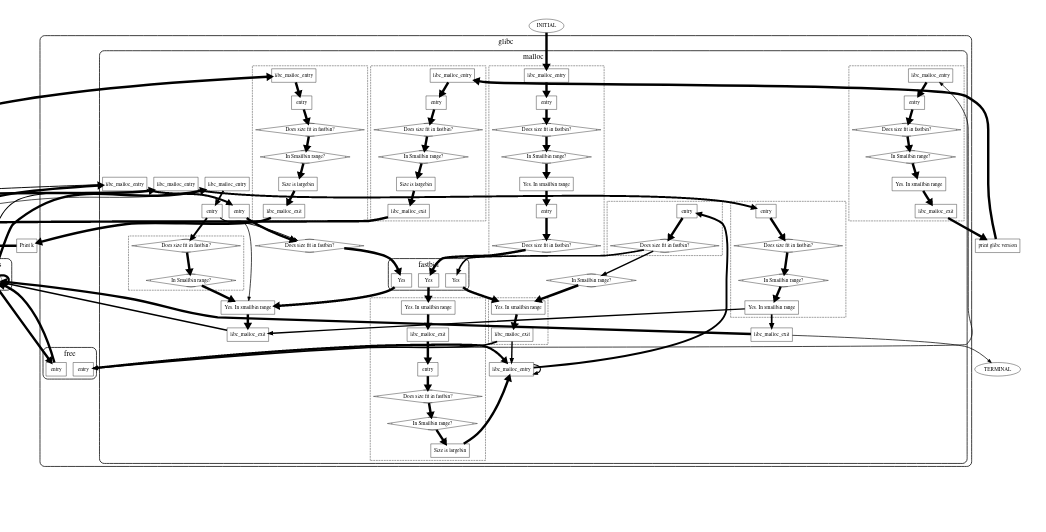
\includegraphics[scale=0.3]{simplification-sequential-on}
\caption{Off/On comparison showing strictly sequential grouping}
    \label{fig:seq-on-off}
\end{figure}
